\doublespacing % Do not change - required

\chapter{Experiments and Results}
\label{ch:experiments}

%%%%%%%%%%%%%%%%%%%%%%%%%%%%%%%%%%%%%%%
% IMPORTANT
\begin{spacing}{1} %THESE FOUR
\minitoc % LINES MUST APPEAR IN
\end{spacing} % EVERY
\thesisspacing % CHAPTER
% COPY THEM IN ANY NEW CHAPTER
%%%%%%%%%%%%%%%%%%%%%%%%%%%%%%%%%%%%%%%

This chapter reports the empirical evaluation of the governance bot.  A controlled experiment was carried out with ten participants to compare a standard plurality rule with a weighted token‑allocation method in a ``Day~Out'' planning scenario.  Participants completed pre‑ and post‑surveys, cast ballots in both voting conditions and provided qualitative feedback.  The following sections describe the experimental setup, summarise the participant cohort, analyse the survey data, compare the voting outcomes and highlight qualitative themes.

\section{Experimental Setup}

Ten participants were recruited through personal networks and invited to join a dedicated Discord server.  All provided informed consent and completed a pre‑voting survey capturing demographic information and attitudes toward fairness and speed in decision‑making.  The core of the experiment was a multi‑stage ``Day~Out'' planning task in which the group had to choose a breakfast, transport, hangout location, lunch, afternoon activity, dinner and late‑night plan.  Two voting mechanisms were implemented:

\begin{enumerate}
    \item \textbf{Plurality voting}: participants cast a single vote for their preferred option in each category.  Votes were counted using a plurality rule, and the option with the most votes won.
    \item \textbf{Weighted voting}: participants were endowed with a budget of fourteen tokens (as described in Section~\ref{sec:token-allocation}) and allocated these tokens across the options in each category to express the strength of their preferences.  Tokens could be split among alternatives, and the option with the highest total token investment in each category was selected.
\end{enumerate}

The order of conditions was counterbalanced to mitigate order effects.  After completing both voting sessions, participants filled out a post‑voting survey assessing how fair and satisfying they found each outcome, whether the process reflected the group’s preferences, whether they would reuse the method and which voting method they would prefer to use in future decisions.  Open‑ended questions invited suggestions for improvement.

\section{Participant Summary}

The cohort comprised ten volunteers (five female and five male) with a mean age of around twenty‑five.  Most were active Discord users: nine of ten reported having used Discord before, but only half had heard of plurality voting, and only four had prior awareness of weighted voting mechanisms.  On a five‑point scale (1\,=\,strongly agree to 5\,=\,strongly disagree), respondents on average leaned toward caring that a decision feels fair to the group ($\mu = 2.6$) and were relatively neutral regarding speed versus fairness ($\mu = 2.9$).  These responses indicate a general openness to more expressive voting methods.

\section{Survey Results}

Table~\ref{tab:survey-results} summarises the mean and standard deviation of key post‑survey items for each voting condition.  Participants rated the extent to which the process reflected the group’s preferences (a proxy for perceived fairness), their satisfaction with the outcome, and whether they would reuse the process in their own groups.  Ratings were given on a five‑point Likert scale.

\begin{table}[h]
    \centering
    \caption{Mean ($\mu$) and standard deviation ($\sigma$) of post‑survey responses on a five‑point scale.  Higher scores indicate greater agreement.}
    \label{tab:survey-results}
    \begin{tabular}{lcc}
        \toprule
        \textbf{Metric} & \textbf{Plurality voting} & \textbf{Weighted voting} \\ \midrule
        Process reflects group preferences & $(\mu=3.9,\;\sigma=0.99)$ & $(\mu=4.3,\;\sigma=1.06)$ \\
        Satisfaction with outcome & $(\mu=3.8,\;\sigma=0.92)$ & $(\mu=4.4,\;\sigma=1.07)$ \\
        Would reuse the process & $(\mu=4.0,\;\sigma=0.82)$ & $(\mu=4.5,\;\sigma=0.85)$ \\ \bottomrule
    \end{tabular}
\end{table}

The results, summarised in Table~\ref{tab:survey-results} and visualised in Figure~\ref{fig:bar-comparison}, show that across all three items the weighted voting condition achieved higher mean scores.  Participants felt that the token‑allocation method better captured group preferences and were more satisfied with the resulting plan.  They also expressed a stronger willingness to reuse the weighted process in future decisions.  The differences of roughly half a point on the five‑point scale are notable given the small sample.

Beyond these quantitative ratings, the post‑survey included several categorical questions.  Seven out of ten participants indicated that they would prefer to use weighted voting in similar situations, while the remaining three expressed a preference for weighted voting once they become more comfortable with the interface.  None favoured the standard plurality rule.  In terms of learning effects, eight participants reported that their understanding of voting methods improved (four ``Much better'', four ``Better''), while two felt it remained the same.  When asked about the cognitive demands of allocating tokens, five agreed and four strongly agreed that the process made them consider their choices more carefully; eight agreed or strongly agreed that they were able to use their tokens effectively; and nine agreed or strongly agreed that the weighted process made them feel their voice was heard more clearly than in the plurality vote.  These responses suggest that, despite the additional step of distributing tokens, participants perceived the expressive mechanism as manageable and beneficial.

\section{Voting Outcomes}

\subsection*{Plurality voting results}

In the plurality voting session the options receiving the highest number of votes (plurality winners) formed the group’s ``Day~Out'' plan:

\begin{itemize}
    \item \emph{Breakfast:} Indian (paratha, dosa, idli) (3 votes)
    \item \emph{Transport:} Car road trip (4 votes)
    \item \emph{Hangout location:} Park/Picnic spot (5 votes)
    \item \emph{Lunch:} Chinese (5 votes)
    \item \emph{Afternoon activity:} Sports (4 votes)
    \item \emph{Dinner:} Fancy restaurant (6 votes)
    \item \emph{Late‑night finish:} Dessert outing (4 votes)
\end{itemize}

All categories were decided by clear pluralities.  The plan balanced active and relaxing activities, with the afternoon spent playing sports and the evening culminating in a fancy dinner and a dessert outing.

\subsection*{Weighted voting results}

For the weighted vote, token allocations were summed across participants for each option.  The resulting plan was mostly consistent with the plurality outcome:

\begin{itemize}
    \item \emph{Breakfast:} Indian (paratha, dosa, idli) (9 tokens)
    \item \emph{Transport:} Car road trip (10 tokens)
    \item \emph{Hangout location:} Park/Picnic spot (12 tokens)
    \item \emph{Lunch:} Chinese (10 tokens)
    \item \emph{Afternoon activity:} Museum/Gallery (12 tokens)
    \item \emph{Dinner:} Fancy restaurant (13 tokens)
    \item \emph{Late‑night finish:} Dessert outing (7 tokens)
\end{itemize}

Only the afternoon activity differed: whereas sports received the most votes in the plurality session, the museum/gallery option attracted the most tokens.  This shift suggests that some participants had strong but dispersed preferences for visiting a museum, which were captured by the token‑allocation mechanism but muted under plurality voting.  In all other categories the winning options matched the plurality winners, indicating broad consensus.

\section{Qualitative Feedback}

Open‑ended feedback offered additional insight into participants’ experiences.  Several praised the bot’s ease of use and overall concept (``It was great!''), while others suggested minor improvements.  Two respondents noted that the ``token UI could be a bit clearer'' and requested clearer instructions on how to allocate tokens.  One simply wrote ``Good effort''.  No participant expressed negative sentiments about the mechanism itself.  Overall, the qualitative data underscore that participants appreciated the opportunity to express the strength of their preferences and that improving the clarity of the token interface could further enhance usability.

\section{Visualisation}

Figure~\ref{fig:bar-comparison} provides a visual comparison of the mean survey ratings across the two conditions.  The grouped bar chart highlights the consistently higher scores achieved by weighted voting on all three metrics.

\begin{figure}[h]
    \centering
    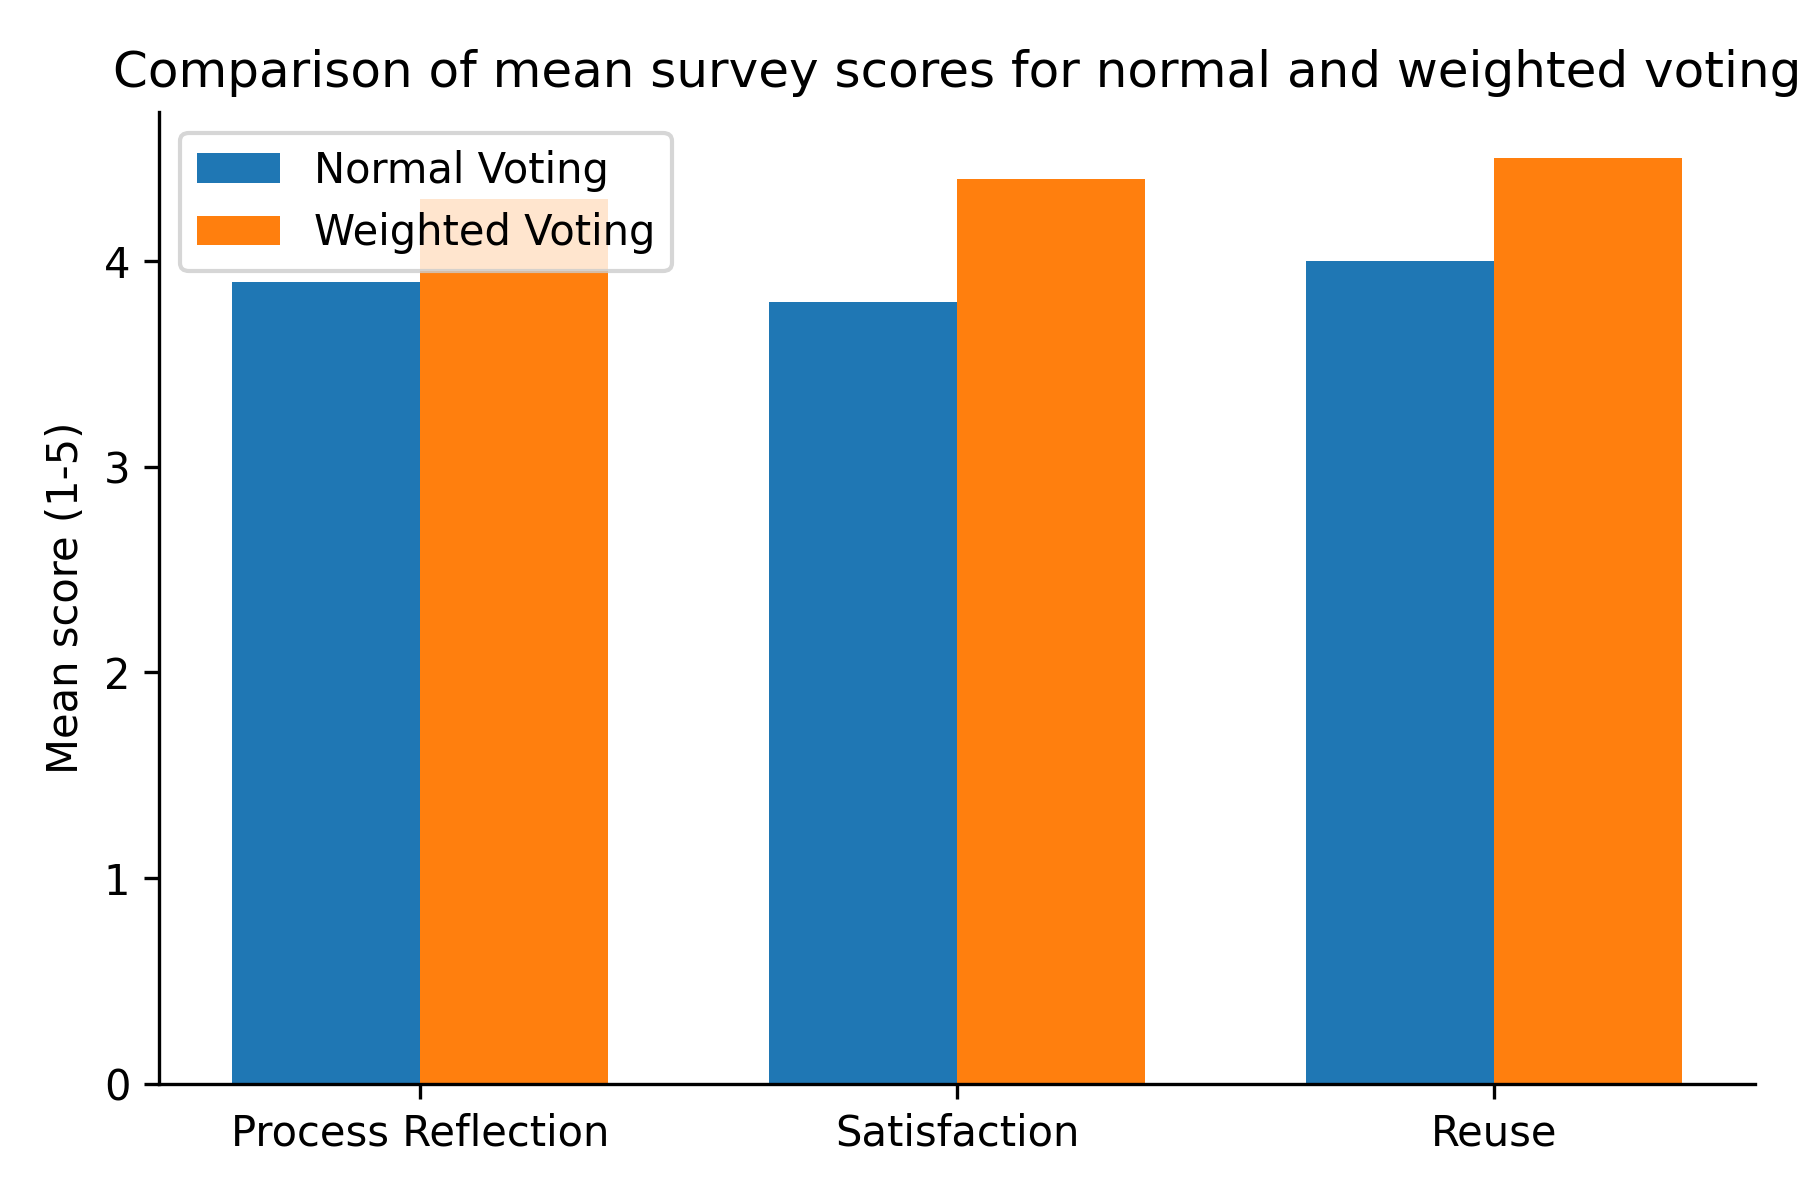
\includegraphics[width=0.8\linewidth]{imgs/token_comparison_chart.png}
    \caption{Comparison of mean survey ratings between plurality and weighted voting.  }
    \label{fig:bar-comparison}
\end{figure}

Taken together, these results indicate that allowing participants to allocate tokens not only changed one component of the ``Day~Out'' plan but also improved perceptions of fairness and satisfaction.  Participants overwhelmingly preferred the weighted method for future decisions, even while noting that the token interface could be refined.  The next chapter interprets these findings in relation to the broader literature on social choice and PD.